% !TEX root = Theo_III.tex

\chapter{Einleitung\label{ref-001}}

\section{Geschichte\label{ref-002}}

\textbf{1864} \textendash{} James Clerk Maxwell: Maxwell-Gleichungen = Feldgleichungen des elektromagnetischen Feldes

elektrisches Feld $E$ ${\Leftrightarrow}$ magnetische Induktion $B$

Hilfsfelder für Materie: dielektrische Verschiebung $D$ und Magnetfeld $H$

Vakuum: $B=\mu _{0}H, D=\varepsilon _{0}E$
\begin{equation*}
	\nabla \cdot D=\rho ,\nabla \cdot B=0,\nabla \times E=-\partial _{t}B,\nabla \times H=j+\partial _{t}E
\end{equation*}
Vermutung: Licht = elektromagnetische Welle

\textbf{1886} \textendash{} Heinrich Hertz: Nachweis elektromagnetischer Wellen. \textit{Äther} als hypothetisches Ausbreitungsmedium

\textbf{1881} \textendash{} Michelson-Morley-Experiment: Konstanz der Lichtgeschwindigkeit unabhängig von Beobachter und Quelle ${\Rightarrow}$ absolutes Bezugssystem \textit{Äther} existiert nicht.

\textbf{1905} \textendash{} Albert Einstein: spezielle Relativitätstheorie.

\section{Inhalt\label{ref-003}}


\begin{itemize}
	\item Einleitung

	\item Elemente der Vektoranalysis

	\item Elektrostatik

	\item Elektrische Felder in Materie

	\item Magnetostatik

	\item Grundgleichungen der Elektrodynamik: Die Maxwellschen Gleichungen

	\item Spezielle Relativitätstheorie

	\item Ebene elektromagnetische Wellen

	\item Elektromagnetische Felder bei vorgegebenen Ladungen und Strömen


\end{itemize}
\section{Grundlegende Konstanten der Elektrodynamik\label{mark-1.3}}

Für Konstanten deren Wert per Definition festgelegt wurde, wird ein $\equiv $-Zeichen verwendet.


\begin{table}[H]
    \centering
	\begin{tabular}{|c|l|} \hline
		\textbf{Konstante}         & \textbf{Wert} \\\hline
		Vakuumlichtgeschwindigkeit & \centering\arraybackslash{}$c_{0}\equiv 299792458\frac{\mathrm{m}}{\mathrm{s}}$  \\\hline
		Elektrische Feldkonstante  & $\varepsilon _{0}=8,8541878128\left(13\right)\cdot 10^{-12}\frac{\mathrm{As}}{\mathrm{Vm}}$ \\\hline
		Magnetische Feldkonstante  & $\mu _{0}=1,25663706212\left(19\right)\cdot 10^{-6}\frac{\mathrm{N}}{\mathrm{A}^{2}}$  \\\hline
		                           &         \\\hline
	\end{tabular}
\end{table}
\section{Grundlegende Formeln der Elektrodynamik\label{mark-1.4}}

Maxwellsche Feldgleichungen
\begin{equation*}
	\nabla \cdot \vec {D}=\rho _{f},\nabla \cdot \vec {B}=0,\nabla \times \vec {E}=-\frac{\partial \vec {B}}{\partial t},\nabla \times \vec {H}=\vec {j}_{f}+\frac{\partial \vec {D}}{\partial t}
\end{equation*}
Materialgleichungen
\begin{equation*}
	\vec {D}=\varepsilon _{0}\vec {E}+\vec {P}, \vec {B}=\mu _{0}\left(\vec {H}+\vec {M}\right)
\end{equation*}
In linearen und isotropen Medien gilt
\begin{equation*}
	\vec {D}=\varepsilon _{0}\varepsilon _{r}\vec {E}, \vec {B}=\mu _{0}\mu _{r}\vec {H}
\end{equation*}
Im Vakuum gilt
\begin{equation*}
	\vec {D}=\varepsilon _{0}\vec {E}, \vec {B}=\mu _{0}\vec {H}
\end{equation*}
Relationen von Lichtgeschwindigkeit, Feldkonstanten und Brechungsindex:

\begin{align*}
	c_{0} & =\frac{1}{\sqrt{\varepsilon _{0}\mu _{0}}} \\
	n     & =\frac{c_{0}}{c}
\end{align*}

In linearen, isotropen Medien gilt
\begin{equation*}
	n=\sqrt{\varepsilon _{0}\mu _{0}}
\end{equation*}
Gradient
\begin{equation*}
	\nabla \frac{1}{r}=-\frac{\vec {r}}{r^{3}}
\end{equation*}
Elektrisches Potential und elektrisches Feld:
\begin{equation*}
	\vec {E}=-\nabla \phi , \phi \left(\vec {r}\right)=\frac{1}{4\pi \varepsilon _{0}}\int \frac{\rho \left(\vec {r}'\right)}{\left| \vec {r}-\vec {r}'\right| }\diff ^{3}\vec {r}'
\end{equation*}
\chapter{Elemente der Vektoranalysis\label{ref-004}}

\section{Vektoranalysis\label{ref-005}}

\subsection{Gradient und Nabla-Operator\label{ref-006}}

Der Gradient eines skalaren Feldes $U$ ist definiert über das totale Differential:
\begin{equation*}
	\diff U=\grad U\cdot \diff \vec {r}=\nabla U\cdot \diff \vec {r}
\end{equation*}
Der Gradient steht senkrecht auf den Äquipotentiallinien. Für kartesische Koordinaten gilt
\begin{equation*}
	\nabla =\vec {e}_{x}\frac{\partial }{\partial x}+\vec {e}_{y}\frac{\partial }{\partial y}+\vec {e}_{z}\frac{\partial }{\partial z}=\sum _{i}\vec {e}_{i}\nabla _{i},
\end{equation*}
während für krummlinige allgemein gilt, dass
\begin{equation*}
	\nabla =\sum _{i}\vec {e}_{i}\frac{1}{\left| \partial \vec {r}/\partial x_{i}\right| }\frac{\partial }{\partial x_{i}}.
\end{equation*}
\subsection{Divergenz eines Vektorfeldes\label{ref-007}}

Die Divergenz eines Vektorfeldes $\vec {a}$ wird beschrieben durch
\begin{equation*}
	\divg \vec {a}\left(\vec {r}\right)=\nabla \cdot \vec {a}\left(\vec {r}\right).
\end{equation*}
Sie gibt die Quellenhaftigkeit von $\vec {a}$ an. In kartesischen Koordinaten ist $\divg \vec {a}=\sum _{i}\nabla _{i}a_{i}$.



\begin{figure}[htb]
	\centering
	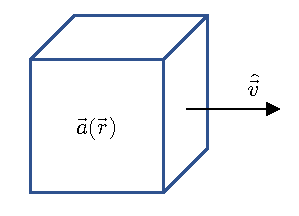
\includegraphics{vecanalysis_flow.pdf}
	\caption{}
	\label{fig:vecanalysis_flow}
\end{figure}

Betrachte zum Verständnis ein kleines Volumen $\Delta  V$ bei $\vec {r}$. Die Normalen $\hat{\vec {\nu }}$ zeigen überall nach außen. Der Fluss aus $\Delta  V$ heraus ist
\begin{equation*}
	q\left(r\right)\Delta  V,
\end{equation*}
wobei $q\left(r\right)=\divg \vec {a}$. Wir können sagen, dass
\begin{align*}
	q\left(\vec {r}\right)=\divg \vec {a}=\begin{cases} >0, & \text{Quelle von }\vec {a}                     \\
              <0, & \text{Senke von }\vec {a}                      \\
              =0, & \text{was reinflie\ss t},\text{flie\ss t raus}
	                                      \end{cases} .
\end{align*}
\subsection{Rotation eines Vektorfeldes\label{ref-008}}

Die Rotation eines Vektorfeldes $\vec {a}$ ist definiert als
\begin{equation*}
	\rot \vec {a}\left(\vec {r}\right)=\nabla \times \vec {a}\left(\vec {r}\right)
\end{equation*}


\begin{figure}[htb]
	\centering
	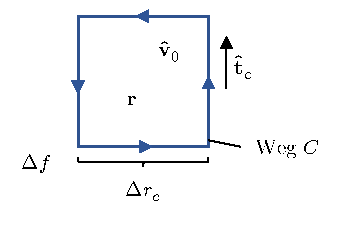
\includegraphics{vecanaylsis_curl.pdf}
	\caption{}
	\label{fig:vecanaylsis_curl}
\end{figure}

und es wird auch als das Wirbelfeld von $\vec {a}$ bezeichnet. Wieder ist die Darstellung in kartesischen Koordinaten einfach: $\left(\rot \vec {a}\right)_{i}=\varepsilon _{ijk}\partial _{{x_{j}}}a_{k}$.

Wir schauen uns ein kleines orientiertes Flächenelement $\Delta  f$ an. Dann ist die Verwirbelung/Zirkulation um $\Delta  f$
\begin{equation*}
	\sum _{C}\vec {a}\cdot \hat{\vec {t}}_{C}\Delta  r_{C}=\rot \vec {a}\cdot \Delta  f
\end{equation*}
mit Tangentialvektor $\hat{\vec {t}}_{C}$ und Parallelkomponente $\vec {a}\cdot \hat{\vec {t}}_{C}$. Wir bezeichnen $\vec {\omega }=\rot \vec {a}$ als lokale Wirbelstärke.

Allgemein gilt, dass Gradientenfelder wirbelfrei sind,
\begin{equation*}
	\vec {a}=\grad U\Leftrightarrow \rot \vec {a}=0\quad\mathrm{bzw.}\quad  \rot \left(\grad U\right)=0
\end{equation*}
und Wirbelfelder quellenfrei sind,
\begin{equation*}
	\divg \vec {B}=0\Leftrightarrow \vec {B}=\rot \vec {A}\quad\mathrm{bzw.}\quad  \divg \left(\rot \vec {A}\right)=0.
\end{equation*}
Wir definieren ferner den Laplace-Operator als
\begin{equation*}
	\Delta  \equiv \nabla ^{2}\equiv \nabla \cdot \nabla ,
\end{equation*}
für den in kartesischen Koordinaten gilt:
\begin{equation*}
	\nabla ^{2}=\partial _{x}^{2}+\partial _{y}^{2}+\partial _{z}^{2}.
\end{equation*}
\subsection{Fundamentalsatz der Vektoranalysis (Helmholtz-Theorem)\label{ref-009}}

Das Helmholtz-Theorem besagt, dass Quellen und Wirbel ein Vektorfeld $\vec {a}\left(\vec {r}\right)$ eindeutig bestimmen. Ein Vektorfeld kann also in ein Rotationsfeld und ein Wirbelfeld aufgeteilt werden:
\begin{equation*}
	\vec {a}=\underset{\substack{
		    \omega =\rot \vec {a}=\rot \vec {a}_{t} \\
			\divg \vec {a}_{t}=0 \\
			\text{Wirbel}!
		}}{\underbrace{\vec {a}_{t}}}+\underset{\substack{
			\rho =\divg \vec {a}=\divg \vec {a}_{l} \\
			\rot \vec {a}_{l}=0                     \\
			\text{Quellen}!
        }}{\underbrace{\vec {a}_{l}}}+\underset{\substack{
			\rot \vec {a}_{r}=\divg \vec {a}_{r}=0 \\
			\text{Randbedingungen}                 \\
			\hat{\vec {\nu }}\cdot \vec {a}=f\left(\vec {r}\right),\vec {r}\in \partial V
	}}{\underbrace{\vec {a}_{r}}}
\end{equation*}
Eine zusätzliche, sowohl quellen- als auch wirbelfreie Komponente kann vorkommen, um Randbedingungen zu erfüllen oder einen konstanten Untergrund zu addieren.

Ebene Transversalwellen ($e^{i\vec {k}\cdot \vec {r}}\bot \vec {k}$) sind zum Beispiel quellenfrei, ebene Longitudinalwellen ($e^{i\vec {k}\cdot \vec {r}}\parallel \vec {k}$) sind dagegen wirbelfrei, denn
\begin{equation*}
	\divg \left(e^{i\vec {k}\cdot \vec {r}}\right)=i\vec {k}\cdot e^{i\vec {k}\cdot \vec {r}}, \rot \left(e^{i\vec {k}\cdot \vec {r}}\right)=i\vec {k}\times e^{i\vec {k}\cdot \vec {r}}.
\end{equation*}
\section{Integration von Feldern\label{ref-010}}

\subsection{Linienintegrale\label{ref-011}}


\begin{equation*}
	\int _{C}\vec {a}\left(\vec {r}\right)\cdot \diff \vec {r}=\int _{C}\vec {a}\left(\vec {r}\left(s\right)\right)\cdot \frac{\diff \vec {r}}{\diff s}\diff s
\end{equation*}


\begin{figure}[htb]
	\centering
	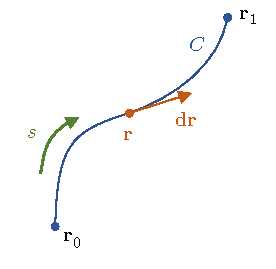
\includegraphics{vecanaylsis_curve.pdf}
	\caption{}
	\label{fig:vecanaylsis_curve}
\end{figure}

Parameterdarstellung: $\vec {r}=\vec {r}\left(s\right)\rightarrow \diff \vec {r}=\frac{\diff \vec {r}}{\diff s}\diff s$ mit der Bogenlänge $s$.

Für rotationsfreie (Einschränkung, siehe Satz von Poincaré) Felder ist das Linienintegral zwischen zwei Punkten wegunabhängig:
\begin{equation*}
	\oint \vec {a}\cdot \diff \vec {r}=0\Leftrightarrow \vec {a}\left(\vec {r}\right)=\nabla \varphi \Leftrightarrow \rot \vec {a}=\vec {0}.
\end{equation*}
\subsection{Satz von Stokes\label{ref-012}}


\begin{equation*}
	\underset{\text{Fluss von }\rot \vec {a}~\text{durch} F}{\underbrace{ \int _{F}\rot \vec {a}\cdot \diff f}}=\underset{\text{Zirkulation von }\vec {a}~\text{entlang}~ C=\partial F}{\underbrace{\oint _{C=\partial F}\vec {a}\cdot \diff \vec {r}}}
\end{equation*}


\begin{figure}[htb]
	\centering
	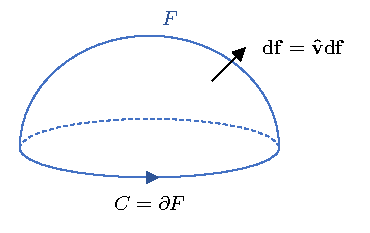
\includegraphics{vecanaylsis_normal.pdf}
	\caption{}
	\label{fig:vecanaylsis_normal}
\end{figure}

Die Kurve $C$ ist dabei stets so orientiert, dass sie der Rechte-Hand-Regel folgt. Von außen (die Seite, nach der der Normalenvektor $\diff \vec {f}$ zeigt) betrachtet geht die Kurve gegen den Uhrzeigersinn.

\subsection{Satz von Gauß\label{ref-013}}


\begin{equation*}
	\underset{\text{Quellen von }\vec {a}~\mathrm{in} V}{\underbrace{ \int _{V}\divg \vec {a}\cdot \mathrm{dV}}}=\underset{\substack{
			\text{Fluss von }\vec {a}~\text{durch } \\
			\partial V \mathrm{aus}~V \text{heraus}
		}}{\underbrace{\int _{\partial V}\vec {a}\cdot \diff f}}
\end{equation*}
Aus den Satz von Gauß abgeleiteten Formen:
\begin{itemize}
	\item $\vec {a}=g\vec {e}_{i}\rightarrow \int _{V}\frac{\partial }{\partial x_{i}}g\diff V=\int _{\partial V}g\diff f_{i}$

	\item $g=a_{j}\rightarrow \int _{V}\rot \vec {a}\diff V=\int _{\partial V}\diff \vec {f}\times \vec {a}$

	\item Greensche Identitäten (diese finden ihre Anwendung in der Potentialtheorie, hierzu wird $\nabla ^{2}\varphi $ verwendet). $\vec {a}_{1}=\varphi \nabla \psi , \vec {a}_{2}=\psi \nabla \varphi $. \begin{enumerate}[a]
		      \setcounter{enumii}{14}

		      \item[o] 1. Identität: $\int \nabla \cdot \vec {a}_{1}\diff V$
			      \begin{equation*}
				      \int _{V}\left(\nabla \varphi \cdot \nabla \psi +\varphi \nabla ^{2}\psi \right)\diff V=\int _{\partial V}\varphi \nabla \psi \cdot \diff f
			      \end{equation*}
		      \item[o] 2. Identität: $\int \left(\nabla \cdot \vec {a}_{1}-\nabla \cdot \vec {a}_{2}\right)\diff V$ (Greenscher Satz)
			      \begin{equation*}
				      \int _{V}\left(\varphi \nabla ^{2}\psi -\psi \nabla ^{2}\varphi \right)\diff V=\int _{\partial V}\left(\varphi \nabla \psi -\psi \nabla \varphi \right)\cdot \diff f
			      \end{equation*}
	      \end{enumerate}

\end{itemize}
\chapter{Elektrostatik\label{ref-014}}

Die Elektrostatik behandelt elektrische Felder ruhender oder langsam bewegter elektrischer Ladungen. In den folgenden Kapiteln werden die Grundgesetze der Elektrostatik aus dem Coulomb-Gesetz abgeleitet.

\section{Bemerkungen zur elektrischen Ladung\label{ref-015}}

Es gibt zwei Arten von Ladungen: positive und negative Ladung. Die Ladung ist eine diskrete Größe und nimmt stets ein ganzzahliges Vielfaches der sogenannten Elementarladung $e_{0}$ an:
\begin{equation*}
	e_{0}=1.602176624\cdot 10^{-19}\,\mathrm{C}
\end{equation*}
Diese wurde zuerst bei dem Millikan-Versuch bestimmt. So trägt zum Beispiel das Proton die Ladung $+e_{0}$ und das Elektron die Ladung $-e_{0}$. Die Quarks haben zwar Bruchteile der Elementarladung, treten aber nie frei, sondern nur in Kombinationen auf, die ein Vielfaches der Elementarladung bilden.

Es gilt strenge Ladungserhaltung:
\begin{quote}

	\begin{quote}
		In einem abgeschlossenen System bleibt die Summe aller Ladungen konstant.
	\end{quote}

\end{quote}
Eine Ladung auf einem infinitesimalen Raum wird als Punktladung bezeichnet. In der Elektrostatik und der Elektrodynamik wird häufig mit der Ladungsdichte $\rho $ gerechnet. Für eine einzige Punktladung $q$ (zum Beispiel ein Proton oder Elektron) am Ort $\vec {r}_{0}$ gilt für die Ladungsdichteverteilung
\begin{equation*}
	\rho \left(\vec {r}\right)=q\delta \left(\vec {r}-\vec {r}_{0}\right).
\end{equation*}
Daraus lässt sich die Ladungsdichte für viele Punktladungen $q_{i}$ an Orten $\vec {r}_{i}$ verallgemeinern:
\begin{equation*}
	\rho \left(\vec {r}\right)=\sum _{i}q_{i}\delta \left(\vec {r}-\vec {r}_{i}\right)
\end{equation*}
Im Grenzwert für kleinste Abstände kann schließlich auch mit kontinuierlichen Ladungsdichten rechnen:
\begin{equation*}
	\rho \left(\vec {r}\right)=\frac{\diff Q}{\diff V}
\end{equation*}
Die gesamte Ladung in einem Volumen $V$ ist also
\begin{equation*}
	Q=\int _{V}\diff ^{3}\vec {r}\rho \left(\vec {r}\right).
\end{equation*}
\section{Coulombsches Gesetz und elektrisches Feld\label{ref-016}}

Im Alllabel machen wir die Erfahrung, dass sich gleichnamige (also zum Beispiel zwei positive) Ladungen abstoßen, während zwischen ungleichnamigen Ladungen eine anziehende Kraft wirkt. Diese Kraft ist ein Vektor im Sinne der Newtonschen Mechanik und unterliegt also dem Superpositionsprinzip.

\subsection{Coulombsches Gesetz\label{ref-017}}

Die Kraft, die eine Ladung $q_{2}$ am Ort $\vec {r}_{2}$ auf eine Ladung $q_{1}$ am Ort $\vec {r}_{1}$ ausübt, berechnet sich durch
\begin{equation}
	\label{3.1}
	\boxed{\vec {F}_{1}=kq_{1}q_{2}\frac{\vec {r}_{1}-\vec {r}_{2}}{\left| \vec {r}_{1}-\vec {r}_{2}\right| ^{3}}=-\vec {F}_{2}}
\end{equation}
Dieses Gesetz wurde experimentell gefunden. Die Proportionalitätskonstante $k$ ist dabei
\begin{equation*}
	k=\frac{1}{4\pi \varepsilon _{0}}
\end{equation*}


\begin{figure}[htb]
	\centering
	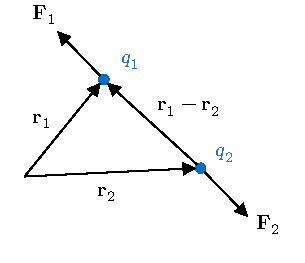
\includegraphics{coulomb_point_charges.pdf}
	\caption{}
	\label{fig:coulomb_point_charges}
\end{figure}

mit Dielektrizitätskonstante $\varepsilon _{0}\approx 8,854\cdot 10^{-12}\,\frac{\mathrm{F}}{\mathrm{m}}$. Das Coulombsche Gesetz hat die gleiche Form wie das Newtonsche Gravitationsgesetz, aber hier kann die Kraft auch abstoßend wirken, weil die Ladung anders als die Masse negativ sein kann. Genauso wie beim Gravitationsgesetz ist die Kraft antiproportional zum Quadrat des Abstands der Ladungen.\footnote{Es ist möglich, dass die Proportionalität nicht exakt $\vec {F}\propto r^{-2}$ ist, aber es ist durch Experimente bestätigt worden, dass für einen Ansatz $F\propto r^{-2-\varepsilon }$ zumindest $\varepsilon <3\cdot 10^{-16}$ ist und für einen Ansatz $F\propto e^{-\frac{r}{\xi }}r^{-2}$ (siehe sogenanntes Yukawa-Potential) wenigstens $\xi >10^{8}\,\mathrm{m}$. }

Mithilfe des Coulombschen Gesetzes können wir nach dem Superpositionsprinzip die Kraft auf eine Testladung $q_{0}$ am Ort $\vec {r}_{0}$ durch mehrere Ladungen $q_{i}$ bestimmen:
\begin{equation}
	\label{3.2}
	\vec {F}=\frac{q_{0}}{4\pi \varepsilon _{0}}\sum _{i}q_{i}\frac{\vec {r}_{0}-\vec {r}_{i}}{\left| \vec {r}_{0}-\vec {r}_{i}\right| ^{3}}
\end{equation}
Dieser Ansatz ist der Fernwirkungsstandpunkt (die Kraft wirkt über die Ferne hinweg).

Beim Nahwirkungsstandpunkt betrachtet man ein elektrisches Feld $\vec {E}$, dass durch Ladungen $q_{i}$ erzeugt wird ($\vec {E}$ zeigt weg von positiven Ladungen und hin zu den negativen):
\begin{equation*}
	\vec {E}\left(\vec {r}\right)=\frac{1}{4\pi \varepsilon _{0}}\sum _{i}q_{i}\frac{\vec {r}_{0}-\vec {r}_{i}}{\left| \vec {r}_{0}-\vec {r}_{i}\right| ^{3}}, \vec {E}\left(\vec {r}\right)=\frac{1}{4\pi \varepsilon _{0}}\int \rho \left(\vec {r}'\right)\frac{\vec {r}-\vec {r}'}{\left| \vec {r}-\vec {r}'\right| ^{3}}\diff ^{3}\vec {r}'
\end{equation*}
Damit ergibt sich die folgende Kraft auf eine Testladung $q_{0}$:
\begin{equation*}
	\vec {F}=q_{0}\vec {E}\left(\vec {r}_{0}\right)
\end{equation*}
\section{Feldgleichungen der Elektrostatik\label{ref-018}}

\subsection{Grundlagen\label{ref-019}}

Wir definieren zunächst das elektrostatische Potential:
\begin{equation}
	\label{3.3}
	\boxed{\vec {E}=-\nabla \phi , \phi \left(\vec {r}\right)=\frac{1}{4\pi \varepsilon _{0}}\int \frac{\rho \left(\vec {r}'\right)}{\left| \vec {r}-\vec {r}'\right| }\diff ^{3}\vec {r}'}
\end{equation}
Weil $\vec {E}$ ein Potentialfeld ist, ist $\rot \vec {E}=0$. Das elektrostatische Feld ist also wirbelfrei.

Beispiel: Potential einer Punktladung:

Das Potential einer Punktladung $\rho \left(\vec {r}\right)=q\delta \left(\vec {r}-\vec {r}_{0}\right)$ ist nach obiger Formel sehr einfach zu berechnen\footnote{Hinweis: Es gilt
	\begin{equation*}
		\nabla \frac{1}{\left| \vec {r}-\vec {r}\mathrm{'}\right| }=-\frac{1}{\left| \vec {r}-\vec {r}\mathrm{'}\right| ^{2}}\nabla \left| \vec {r}-\vec {r}\mathrm{'}\right| \overset{\nabla r=\frac{\vec {r}}{r}=\hat{\vec {r}}}{=}-\frac{\vec {r}-\vec {r}\mathrm{'}}{\left| \vec {r}-\vec {r}\mathrm{'}\right| ^{3}}
	\end{equation*}
}:
\begin{equation*}
	\phi \left(\vec {r}\right)=\frac{1}{4\pi \varepsilon _{0}}\frac{q}{\left| \vec {r}-\vec {r}_{0}\right| }
\end{equation*}
Die Quellen des elektrischen Feldes werden mit der Divergenz berechnet,
\begin{equation*}
	\divg \vec {E}=-\nabla ^{2}\phi =-\frac{1}{4\pi \varepsilon _{0}}\int \rho \left(\vec {r}\mathrm{'}\right)\underset{\overset{!}{=}-4\pi \delta \left(\vec {r}-\vec {r}\mathrm{'}\right)}{\underbrace{\nabla ^{2}\frac{1}{\left| \vec {r}-\vec {r}\mathrm{'}\right| }}}\diff ^{3}r\mathrm{'}=\frac{1}{\varepsilon _{0}}\rho \left(\vec {r}\right).
\end{equation*}
\subsection{Feldgleichungen der Elektrostatik\label{ref-020}}

Die soeben gefundenen Zusammenhänge werden als Feldgleichungen der Elektrostatik bezeichnet:

\begin{align}
	\label{3.4}
	\boxed{\divg \vec {E}=\frac{1}{\varepsilon _{0}}\rho \left(\vec {r}\right)} \\
	\label{3.5}
	\boxed{\rot \vec {E}=0}
\end{align}

Die erste Gleichung wird als Gaußsches Gesetz bezeichnet und beschreibt die elektrische Ladung als Quelle des elektrischen Feldes. Die zweite beschreibt die Wirbelfreiheit des elektrostatischen Feldes.

Mit $\vec {D}=\varepsilon _{0}\vec {E}$ im Vakuum kann man das Gaußsche Gesetz auch umformulieren:
\begin{equation}
	\label{3.6}
	\divg \vec {D}=\rho \left(\vec {r}\right)
\end{equation}
Zu beiden Feldgleichungen gibt es integrale Formulierungen:
\begin{equation*}
	\int _{V}\divg \vec {E}\diff ^{3}r=\int _{\partial V}\vec {E}\cdot \diff \vec {f}=\frac{1}{\varepsilon _{0}}\int \rho \left(\vec {r}\right)\diff ^{3}r\Rightarrow \boxed{\int _{\partial V}\vec {E}\cdot \diff f=\frac{1}{\varepsilon _{0}}Q}
\end{equation*}
Der Fluss aus dem Volumen $V$ heraus ist also proportional zu der Gesamtladung. Betrachte als Beispiel eine Punktladung, die das Feld $\vec {E}=\frac{1}{4\pi \varepsilon _{0}}q\frac{\vec {r}-\vec {r}_{0}}{\left| \vec {r}-\vec {r}_{0}\right| ^{3}}=\frac{1}{4\pi \varepsilon _{0}}q\frac{\hat{\vec {R}}}{R^{2}}$ erzeugt:
\begin{equation*}
	\int _{\partial V_{K}}\vec {E}\cdot \diff \vec {f}=\frac{q}{4\pi \varepsilon _{0}}\int _{\partial V_{K}}\frac{\hat{\vec {R}}}{R^{2}}\cdot \hat{\vec {R}}R^{2}\diff \Omega  =\frac{q}{4\pi \varepsilon _{0}}\int _{\partial V_{K}}\diff \Omega  =\frac{q}{\varepsilon _{0}}
\end{equation*}
Für die andere Feldgleichung betrachten wir das Arbeitsintegral, also die von einer Punktladung $q$ verrichtete Arbeit gegen die elektrische Kraft $F_{\mathrm{el}}=q\vec {E}$.
\begin{equation*}
	W=-q\int _{C}\vec {E}\cdot \diff \vec {r}=q\int _{C}\nabla \phi \cdot \diff \vec {r}=q\int _{C}\diff \phi =q\left[\phi \left(2\right)-\phi \left(1\right)\right]
\end{equation*}
Insbesondere gilt
\begin{equation}
	\label{3.7}
	\oint \vec {E}\cdot \diff \vec {r}=0
\end{equation}

\begin{quote}

	\begin{quote}
		Die Feldlinien des elektrostatischen Feldes sind nicht geschlossen, es gibt keine Zirkulation in der Elektrostatik, $\rot \vec {E}=0$.
	\end{quote}

\end{quote}
\subsection{Potentialgleichung\label{ref-021}}

Aus dem Gaußschen Gesetz können wir die folgende Poisson-Gleichung ableiten, die für $\rho =0$ zu einer Laplace-Gleichung wird:
\begin{equation}
	\label{3.8}
	\boxed{\nabla ^{2}\phi =-\frac{1}{\varepsilon _{0}}\rho }
\end{equation}
Zur Lösung einer linearen Differentialgleichung können wir die Methode der Greenschen Funktion verwenden. Dabei drücken wir die Lösung allgemein als Faltung der Ladungsdichte mit einer sogenannten Greenschen Funktion aus,
\begin{equation}
	\label{3.9}
	\phi \left(\vec {r}\right)=\int G\left(\vec {r}-\vec {r}'\right)\rho \left(\vec {r}'\right)\diff ^{3}\vec {r}'.
\end{equation}
Durch Vergleich mit der Bestimmungsgleichung des elektrischen Potentials können wir die Greensche Funktion für diese Differentialgleichung ablesen:
\begin{equation}
	\label{3.10}
	G\left(\vec {r}-\vec {r}'\right)=\frac{1}{4\pi \varepsilon _{0}}\frac{1}{\left| \vec {r}-\vec {r}'\right| }
\end{equation}
Insbesondere gilt für eine Punktladung $\rho \left(\vec {r}\right)=\delta \left(\vec {r}-\vec {r}_{0}\right)$, dass $\phi \left(\vec {r}\right)=G\left(\vec {r}-\vec {r}_{0}\right)$ und damit, dass
\begin{equation*}
	\nabla ^{2}\frac{1}{\left| \vec {r}-\vec {r}_{0}\right| }=-4\pi \delta \left(\vec {r}-\vec {r}_{0}\right).
\end{equation*}
\subsection{Feldlinien\label{ref-022}}



\begin{figure}[htb]
	\centering
	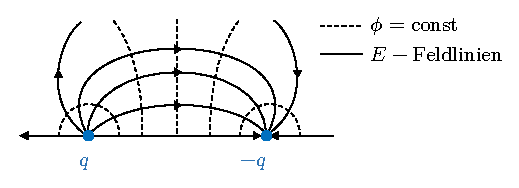
\includegraphics{dipole_field_potential.pdf}
	\caption{}
	\label{fig:dipole_field_potential}
\end{figure}

Als Äquipotentiallinien bzw. -flächen werden die Linien/Flächen gleichen Potentials, $\phi =\text{const}$ bezeichnet. Die Feldlinien stehen senkrecht auf den Äquipotentialflächen, weil $\vec {E}\left(\vec {r}\right)=-\nabla \phi $.

\subsection{Elektrostatische Energie\label{ref-023}}

Die potentielle Energie einer Ladung $q$ am Ort $\vec {r}$ im Feld $\vec {E}=-\nabla \phi $ ist definiert über einen Referenzpunkt $\phi _{1}=0$, der zum Beispiel im Unendlichen liegt:
\begin{equation}
	\label{3.11}
	U\left(\vec {r}\right)=q\phi \left(\vec {r}\right)
\end{equation}
Zum Beispiel ist die potentielle Energie von zwei Punktladungen
\begin{equation*}
	U=q_{1}\phi _{2}=\frac{1}{4\pi \varepsilon _{0}}\frac{q_{1}q_{2}}{\left| \vec {r}_{1}-\vec {r}_{2}\right| }.
\end{equation*}
Die elektrostatische Energie $U$ von $n$ Punktladungen im eigenen Feld kann dann in zwei Schritten bestimmt werden.
\begin{itemize}
	\item Bestimme die Energie von $q_{i}$ im Feld von $q_{j}$ ($j=1,\ldots ,i-1$):
	      \begin{equation*}
		      U_{i}\left(\vec {r}_{i}\right)=q_{i}\sum _{j=1}^{i-1}\phi _{j}=\frac{q_{i}}{4\pi \varepsilon _{0}}\sum _{j=1}^{i-1}\frac{q_{j}}{\left| \vec {r}_{i}-\vec {r}_{j}\right| }
	      \end{equation*}
	\item Bringe $N$ Ladungen sukzessive an ihren Ort:
	      \begin{equation*}
		      U=\sum _{i=2}^{N}U_{i}\left(\vec {r}_{i}\right)=\frac{1}{4\pi \varepsilon _{0}}\sum _{i=2}^{N}\sum _{j=1}^{i-1}\frac{q_{i}q_{j}}{\left| \vec {r}_{i}-\vec {r}_{j}\right| }=\frac{1}{8\pi \varepsilon _{0}}\sum _{i\neq j}^{N}\frac{q_{i}q_{j}}{\left| \vec {r}_{i}-\vec {r}_{j}\right| }
	      \end{equation*}

\end{itemize}
Für eine kontinuierliche Ladungsverteilung ergibt sich
\begin{equation*}
	U=\frac{1}{8\pi \varepsilon _{0}}\int \diff ^{3}\vec {r}\diff ^{3}\vec {r}'\frac{\rho \left(\vec {r}\right)\rho \left(\vec {r}'\right)}{\left| \vec {r}-\vec {r}'\right| }=\frac{1}{2}\int \diff ^{3}\vec {r}\rho \left(\vec {r}\right)\phi \left(\vec {r}\right)
\end{equation*}
Bemerkungen:
\begin{itemize}
	\item Den zusätzlichen Faktor von $\frac{1}{2}$ erhält man, weil $\phi \left(\vec {r}\right)$ von $\rho \left(\vec {r}\right)$ selbst erzeugt wird.

	\item Für beschränkte $\rho $ ist $\vec {r}\rightarrow \vec {r}'$ wohl definiert, da $\diff ^{3}r=r^{2}\diff r\diff \Omega  $


\end{itemize}
Es ist auch möglich, die Energie durch das Feld $\vec {E}\left(\vec {r}\right)$ auszudrücken:
\begin{equation*}
	U=\frac{\varepsilon _{0}}{2}\int \diff ^{3}\vec {r}\phi \nabla ^{2}\phi \overset{\text{partielle Int}.}{=}\frac{\varepsilon _{0}}{2}\int \diff ^{3}\vec {r}\nabla \phi \cdot \nabla \phi =\frac{\varepsilon _{0}}{2}\int \diff ^{3}\vec {r}\left| \vec {E}\right| ^{2}
\end{equation*}
Damit lässt sich die Energiedichte in der Elektrostatik folglich schreiben als
\begin{equation*}
	u\left(\vec {r}\right)=\frac{\varepsilon _{0}}{2}\left| \vec {E}\left(\vec {r}\right)\right| ^{2}=\frac{1}{2}\vec {E}\cdot \vec {D}
\end{equation*}
\subsection{Homogen geladene Kugel\label{ref-024}}



\begin{figure}[htb]
	\centering
	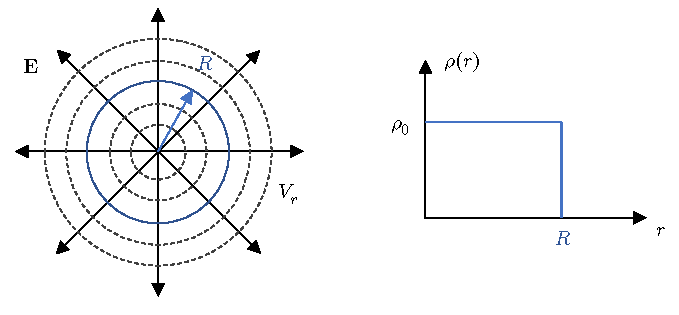
\includegraphics{homogenously_charged_ball.pdf}
	\caption{}
	\label{fig:homogenously_charged_ball}
\end{figure}

Auf der homogen geladenen Kugel $V_{r}$ ist die Ladungsdichte $\rho \left(\vec {r}\right)$ innerhalb der Kugel konstant $\rho _{0}$ und außerhalb der Kugel gleich $0$. Das Problem ist kugelsymmetrisch und hängt nur von der Radialrichtung ab.



\begin{figure}[htb]
	\centering
	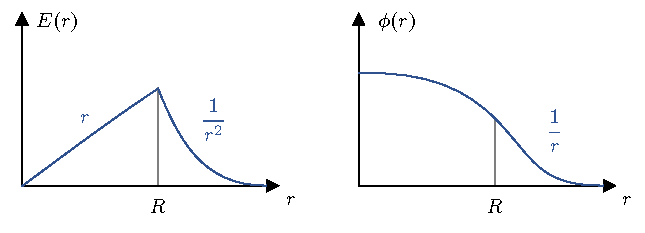
\includegraphics{homogenously_charged_ball_field_potential.pdf}
	\caption{}
	\label{fig:homogenously_charged_ball_field_potential}
\end{figure}

Feld und Potential können zum Beispiel über das Gaußsche Gesetz berechnet werden:
\begin{align*}
		\int _{{V_{r}}}\diff ^{3}r'\frac{\rho \left(r\right)}{\varepsilon _{0}}&=\int _{{V_{r}}}\diff ^{3}r'\divg \vec {E}=\int _{\partial {V_{r}}}\vec {E}\cdot \diff \vec {f}\Rightarrow 4\pi r^{2}E\left(r\right)=\frac{1}{\varepsilon _{0}}\int _{0}^{r}\diff r'r'^{2}\rho \left(r'\right) \\
		\Rightarrow E\left(r\right)&=\frac{Q}{4\pi \varepsilon _{0}}\begin{cases} \frac{r}{R^{2}}, & r<R     \\
              \frac{1}{r^{2}}, & r\geq R
		                                                           \end{cases} \quad\xrightarrow{\text{Integration}}\quad \phi \left(r\right)=\frac{Q}{4\pi \varepsilon _{0}}\begin{cases} \frac{1}{R}\left(\frac{3}{2}-\frac{r^{2}}{2R^{2}}\right), & r<R     \\
              \frac{1}{r},                                              & r\geq R
		                                                                                                                                                                     \end{cases}
\end{align*}
Bemerkenswert ist, dass für $r\geq R$ das elektrische Feld $\vec {E}\left(\vec {r}\right)=E\left(r\right)\cdot \vec {e}_{r}$ gerade dem Feld einer Punktladung $Q$ im Mittelpunkt der Kugel entspricht.

Es soll nun die Energiedichte $u\left(\vec {r}\right)$ für die homogen geladene Kugel berechnet werden:
\begin{align*}
	u\left(\vec {r}\right)=\frac{\varepsilon _{0}}{2}\left| \vec {E}\right| ^{2}=\frac{Q^{2}}{32\pi ^{2}\varepsilon _{0}}\begin{cases} \frac{r^{2}}{R^{6}}, & r<R     \\
              \frac{1}{r^{4}},     & r\geq R
	                                                                                                                     \end{cases}
\end{align*}
Daraus ergibt sich die elektrostatische Energie ("`Selbstenergie`` einer homogen geladenen Kugel)
\begin{equation*}
	U=4\pi \int _{0}^{\infty }\diff ru\left(r\right)r^{2}=\frac{1}{4\pi \varepsilon _{0}}\frac{3}{5}\frac{Q^{2}}{R}.
\end{equation*}
Diese Rechnung lässt eine Abschätzung für den Elektronenradius zu (sogenannter klassischer Elektronenradius):
\begin{equation*}
	U\overset{!}{=}\underset{\text{Ruheenergie von }e^{-}}{\underbrace{m_{e}c^{2}}}\approx 0.5\,\text{MeV }\Rightarrow R_{e}=1,7\cdot 10^{-15}\,\mathrm{m}
\end{equation*}
Allerdings liegt die Compton-Wellenlänge $\lambda _{e}=\frac{h}{m_{e}c}=2\cdot 10^{-12}\,\mathrm{m}$ schon weit über diesem Radius, sodass Quanteneffekte hier nicht vernachlässigbar sind.

\subsection{Extremalprinzip und Kapazitäten\label{ref-025}}


\begin{quote}

	\begin{quote}
		In der Elektrostatik sind Leiter stets Äquipotentialflächen, d.h. $\phi =\text{const}$ und daher $\vec {E}=-\nabla \phi =\vec {0}$ entlang des Leiters. Sonst würde ein Strom fließen, weil sich die freien Elektronen im Leiter aufgrund des nicht-verschwindenden Feldes bewegen würden.
	\end{quote}

\end{quote}


\begin{figure}[htb]
	\centering
	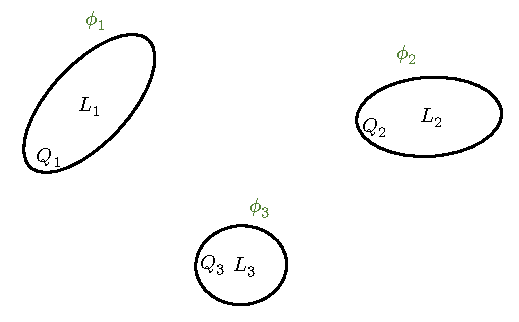
\includegraphics{three_conductors.pdf}
	\caption{}
	\label{fig:three_conductors}
\end{figure}

Betrachte den Fall von $n$ Leitern mit Volumina $L_{i}$, einer Ladung $Q_{i}$ und den Potentialen $\phi _{i}$.

Es soll untersucht werden, wie aus der Ladungsverteilung die Potentiale und das elektrische Feld bestimmt werden können.
\begin{quotation}

	\begin{quote}
		\textbf{\textup{Theorem von Thomson:}}
	\end{quote}

	\begin{quote}
		Die Ladungsdichten $\rho _{i}\left(\vec {r}\right)$ in Leitern $i$ stellen sich so ein, dass die Gesamtenergie minimal wird.
	\end{quote}

\end{quotation}
Beweis:
\begin{equation*}
	U=\frac{1}{8\pi \varepsilon _{0}}\sum _{ij}\int _{L_{i}}\diff ^{3}\vec {r}_{i}\int _{L_{j}}\diff ^{3}\vec {r}_{j}\frac{\rho _{i}\left(\vec {r}_{i}\right)\rho _{j}\left(\vec {r}_{j}\right)}{\left| \vec {r}_{i}-\vec {r}_{j}\right| }
\end{equation*}
Minimierung unter der Nebenbedingung $\int _{{L_{i}}}\diff ^{3}\vec {r}\rho _{i}\left(\vec {r}\right)=Q_{i}$ führt auf
\begin{equation*}
	\frac{\partial }{\partial \rho _{k}\left(\vec {r}\right)}\left(U-\sum _{i}\phi _{i}\int _{L_{i}}\diff ^{3}\vec {r}_{i}\rho _{i}\left(\vec {r}\right)\right)=0
\end{equation*}
wobei in Voraussicht die Lagrange-Parameter als $\phi _{i}$ bezeichnet werden, weil sich mit
\begin{equation*}
    \partial _{{\rho _{k}}\left(\vec {r}\right)}\sum _{i}\int \rho _{i}\left(\vec {r}\right)f_{i}\left(\vec {r}\right)\diff ^{3}r=f_{k}\left(\vec {r}\right)
\end{equation*}
ergibt, dass
\begin{equation*}
	\phi _{k}=\frac{1}{4\pi \varepsilon _{0}}\sum _{j}\int _{L_{j}}\diff ^{3}\vec {r}_{j}\frac{\rho _{j}\left(\vec {r}_{j}\right)}{\left| \vec {r}_{k}-\vec {r}_{j}\right| }, \vec {r}_{k}\in L_{k}
\end{equation*}
was gerade der Bestimmungsgleichung für das Potential $\phi _{k}$ als Potential von $L_{k}$ entspricht. Da das Vorgehen der Minimierung der Gesamtenergie auf das richtige Potential führt, ist das Theorem bestätigt.

\subsubsectiona{Kapazitäten\label{ref-026}}

Die Potentiale $\phi _{i}$ lassen sich linear über die Ladungen $Q_{i}$ zerlegen,
\begin{equation*}
	\phi _{i}=\sum _{j}p_{ij}Q_{j},
\end{equation*}
weil einerseits gilt, dass $\nabla ^{2}\phi =-\rho /\varepsilon _{0}$ und andererseits $\phi $ linear in $\rho $ ist. Dieser Zusammenhang lässt sich invertieren,
\begin{equation*}
	Q_{i}=\sum _{j}C_{ij}\phi _{j},
\end{equation*}
wobei dann die Vorfaktoren $C_{ij}$ als Kapazitäten mit der Einheit $\left[C_{ij}\right]=1\,\frac{\mathrm{C}}{\mathrm{V}}=1\,\mathrm{F}$ definiert werden. Aus dem Ausdruck für die elektrostatische Energie
\begin{equation*}
	U=\frac{1}{2}\sum _{i}\underset{Q_{i}=\sum _{j}C_{ij}\phi _{j}}{\underbrace{\int _{L_{i}}\diff ^{3}\vec {r}_{i}\rho _{i}\left(\vec {r}_{i}\right)\phi _{i}}}=\frac{1}{2}\sum _{ij}\phi _{i}C_{ij}\phi _{j}
\end{equation*}
folgt die Symmetrie $C_{ij}=C_{ji}$.

So gilt zum Beispiel für einen Plattenkondensator allgemein
\begin{equation*}
	C=\frac{Q}{V}, U=\frac{1}{2}CV^{2}=\frac{1}{2}QV
\end{equation*}
für einen Plattenkondensator mit parallelen Platten der Fläche $A$ und Abstand $d$
\begin{equation*}
	C=\varepsilon _{0}\varepsilon _{r}\frac{A}{d},
\end{equation*}
für einen Zylinderkondensator der Länge $L$ und mit Radien $r_{1}<r_{2}$
\begin{equation*}
	C=2\pi \varepsilon _{0}\varepsilon _{r}\frac{L}{\ln \frac{r_{2}}{r_{1}}}
\end{equation*}
und schließlich für einen Kugelkondensator mit Radien $r_{1}<r_{2}$
\begin{equation*}
	C=4\pi \varepsilon _{0}\varepsilon _{r}\left(\frac{1}{r_{1}}-\frac{1}{r_{2}}\right)^{-1}=4\pi \varepsilon _{0}\varepsilon _{r}\frac{r_{1}r_{2}}{d}
\end{equation*}


\begin{figure}[htb]
	\centering
	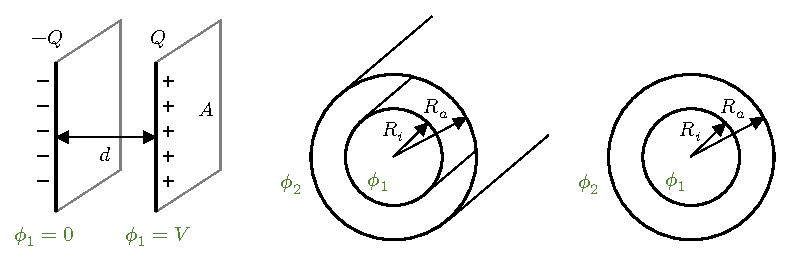
\includegraphics{capacitors.pdf}
	\caption{}
	\label{fig:capacitors}
\end{figure}



\subsection{Maxwellscher Spannungstensor\label{ref-027}}

\section{Randbedingungen des elektrischen Feldes auf Grenzflächen\label{mark-3.4}}

 {\ldots}

\section{Randwertprobleme der Elektrostatik\label{ref-028}}

Meist sind bei der Lösung von elektrostatischen Problemen der Poisson-Gleichung
\begin{equation*}
	\nabla ^{2}\phi =-\frac{\rho }{\varepsilon _{0}}
\end{equation*}
in einem Volumen $V$ noch die Randbedingungen auf $\partial V$ zu berücksichtigen.

\subsection{Eindeutigkeit der Lösung\label{ref-029}}

Allgemein sind drei verschiedene Arten von Randbedingungen möglich. \begin{enumerate}[1)]


	\item[1)] Dirichlet-Randbedingung: Das Potential ist auf dem Rand vorgegeben, $\left.\hspace{0pt}\phi \right| _{\partial V}$.

	\item[2)] Neumann-Bedingungen: Die Normalenableitung der Lösung wird auf dem Rand vorgegeben, $\vec {n}\cdot \left.\hspace{0pt}\nabla \phi \right| _{\partial V}=\left.\frac{\partial \phi }{\partial n}\right| _{\partial V}$

	\item[3)] Cauchy-Bedingungen: $a\left(1\right)+b\left(2\right)$ vorgegeben.

\end{enumerate}
Zum Beispiel kommt die Dirichlet-Randbedingung bei Oberflächen von Leitern vor, von denen wir ja bereits wissen, dass dort das Potential konstant gleich $0$ ist.
\begin{quotation}
	\begin{quote}
		Für Dirichlet- und Neumann-Randbedingungen ist die Lösung der Poisson-Gleichung eindeutig.
	\end{quote}
\end{quotation}
Der Beweis ist einfach, denn seien $\phi _{1}$ und $\phi _{2}$ zwei unterschiedliche Lösungen, dann erfüllt $\phi _{d}=\phi _{1}-\phi _{2}$ die Gleichung $\nabla ^{2}\phi _{2}=0$ mit der Randbedingung
\begin{align*}
	\begin{cases} \left.\phi _{d}\right| _{\partial V}                             & =0 \\
              \left.\frac{\partial \phi _{d}}{\partial n}\right| _{\partial V} & =0
	\end{cases} ,
\end{align*}
da $\phi _{1,2}$ die gleichen Randbedingungen erfüllen. Nach der zweiten Greenschen Identität folgt
\begin{equation*}
	\int _{V}\left(\varphi \nabla ^{2}\psi +\nabla \varphi \cdot \nabla \psi \right)\diff V=\int _{\partial V}\varphi \nabla \psi \cdot \diff \vec {f}.
\end{equation*}
Setze nun $\varphi =\psi =\phi _{d}$:
\begin{equation*}
	\int _{V}\left(\nabla \phi _{d}\right)^{2}\diff V=0
\end{equation*}
Da nun aber der Integrand stets positiv ist. folgt $\nabla \phi _{d}=0$ und also ohne Beschränkung der Allgemeinheit $\phi _{d}=\text{const}=0$.

\subsection{Methode der Greenschen Funktion\label{ref-030}}

\subsection{Aussagen zur Potentialtheorie\label{mark-3.5.3}}

\subsection{Lösungen zur Laplace-Gleichung in Kugelkoordinaten\label{ref-031}}

Die Laplace-Gleichung ist eine zentrale Gleichung in der Physik. In der Elektrostatik gilt sie zum Beispiel im ladungsfreien Raum, aber sie spielt auch für viele andere Modelle eine große Rolle. In kartesischen Koordinaten nimmt die Gleichung die Form
\begin{equation*}
	\nabla ^{2}\phi =\left(\frac{\partial ^{2}}{\partial x^{2}}+\frac{\partial ^{2}}{\partial y^{2}}+\frac{\partial ^{2}}{\partial z^{2}}\right)\phi =0
\end{equation*}
an. Die Lösung lässt sich in Eigenfunktionen des Laplace-Operators zerlegen. Diese sind zum Beispiel für den kartesischen Fall ebene Wellen.

Für kugelsymmetrische Problem bietet es sich an in Kugelkoordinaten zu rechnen. In Kugelkoordinaten lässt sich der Laplace-Operator in Radial- und Winkelanteil zerlegen:
\begin{equation*}
	\nabla ^{2}\phi =\nabla _{r}^{2}\phi +\frac{1}{r^{2}}\nabla _{\varphi ,\vartheta }^{2}\phi =\frac{1}{r^{2}}\frac{\partial }{\partial r}r^{2}\frac{\partial }{\partial r}\phi +\frac{1}{r^{2}\sin \vartheta }\frac{\partial }{\partial \vartheta }\sin \varphi \frac{\partial }{\partial \vartheta }\phi -\frac{1}{r^{2}\sin ^{2} \vartheta }\frac{\partial ^{2}}{\partial \varphi ^{2}}\phi
\end{equation*}
Zur Lösung wird ein Produktansatz gemacht,
\begin{equation*}
	\phi \left(r,\varphi ,\vartheta \right)=R\left(r\right)Y\left(\varphi ,\vartheta \right).
\end{equation*}
Eingesetzt in die Laplace-Gleichung ergibt sich
\begin{equation*}
	Y\nabla _{r}^{2}R+\frac{R}{r^{2}}\nabla _{\varphi ,\vartheta }^{2}Y=0\Leftrightarrow \frac{r^{2}}{R}\nabla _{r}^{2}R=-\frac{1}{Y}\nabla _{\varphi ,\vartheta }^{2}Y=\text{const}
\end{equation*}
Hieraus ergeben sich separat die radialen Eigenfunktionen
\begin{equation*}
	R\left(r\right)=\alpha r^{l}+\beta r^{-\left(l+1\right)}
\end{equation*}
und wie bereits aus der Quantenmechanik bekannt die Kugelflächenfunktionen $Y_{lm}\left(\varphi ,\vartheta \right)$ für den Winkelanteil:
\begin{equation*}
	\nabla _{\varphi ,\vartheta }^{2}Y_{lm}=-l\left(l+1\right)Y_{lm}
\end{equation*}
Die Gesamtlösung setzt sich dann zusammen aus dem Radial- und Winkelanteil:
\begin{equation*}
	\phi \left(r,\varphi ,\vartheta \right)=\sum _{l=0}^{\infty }\sum _{m=-l}^{l}\underset{\text{Radialanteil}}{\underbrace{\left(\alpha _{lm}r^{l}+\beta _{lm}r^{-\left(l+1\right)}\right)}}\underset{\text{Winkelanteil}}{\underbrace{Y_{lm}\left(\varphi ,\vartheta \right)}}
\end{equation*}
Für zylindersymmetrische Probleme ist die $\varphi $-Abhängigkeit aufgehoben und es brauchen nur Funktionen mit $m=0$ betrachtet zu werden.

Für die Kugelflächenfunktionen von zwei Vektoren $\vec {r}_{1}=\left(r_{1},\varphi _{1},\vartheta _{1}\right)$ und $\vec {r}_{2}=\left(r_{2},\varphi _{2},\vartheta _{2}\right)$ gilt das folgende Additionstheorem:
\begin{equation*}
	\sum _{m=-l}^{l}Y_{lm}\left(\varphi _{1},\vartheta _{1}\right)Y_{lm}^{*}\left(\varphi _{2},\vartheta _{2}\right)=\frac{2l+1}{4\pi }P_{l}\left(\cos \angle \left(\vec {r}_{1},\vec {r}_{2}\right)\right)
\end{equation*}
Die Greensche Funktion kann mit diesem Additionstheorem nach den Kugelflächenfunktionen entwickelt werden
\begin{equation*}
	\frac{1}{\left| \vec {r}-\vec {r}'\right| }=\frac{1}{\sqrt{r^{2}+r'^{2}-2rr'\cos \vartheta }}=\sum _{l}\frac{r_{<}^{l}}{r_{>}^{l+1}}P_{l}\left(\cos \vartheta \right), \begin{array}{c}
		r_{>}=\max \left(r,r'\right) \\
		r_{<}=\min \left(r,r'\right)
	\end{array}
\end{equation*}


\begin{figure}[htb]
	\centering
	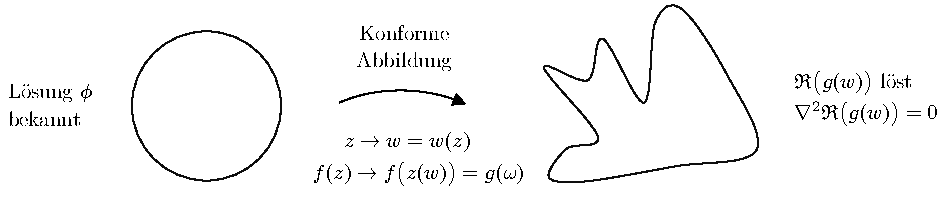
\includegraphics{complex_problems_conformal_map.pdf}
	\caption{}
	\label{fig:complex_problems_conformal_map}
\end{figure}

Obwohl die Wahl der Kugelkoordinaten nur für wenige Probleme sinnvoll ist, kann die Lösung für das kugelförmige Problem durch konforme Abbildungen auf komplexere Geometrien angewandt werden.

\section{Multipolentwicklung\label{ref-032}}

Bei der Multipolentwicklung klassifiziert man bestimmte Ladungsverteilungen nach sogenannten Momenten (Dipolmoment, Quadrupolmoment, {\ldots}). Zum Beispiel beschreibt das Dipolmoment zwei räumlich voneinander getrennte Ladungen unterschiedlichen Vorzeichens. Auch ein nach außen insgesamt elektrisch neutraler Körper kann ein Dipolmoment aufweisen, nämlich wenn die Schwerpunkte von der positiven und negativen Ladung nicht zusammenfallen. Ein prominentes mikroskopisches Beispiel ist das Wassermolekül, bei dem das Sauerstoffatom eine bedeutend größere Elektronegativität besitzt als die Wasserstoffatome und dadurch eine Ladungsverschiebung der gebundenen Elektronen zum Sauerstoffatom hin bewirkt. Dadurch besitzt dieses lokal eine Ladung von $-0.8\,\mathrm{eV}$.

Das Dipolmoment ist ein Vektor und per Definition von der negativen Ladung zur positiven gerichtet



\begin{figure}[htb]
	\centering
	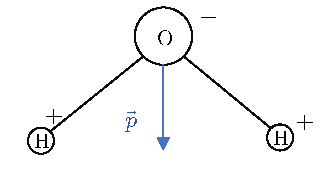
\includegraphics{water_molecule.pdf}
	\caption{}
	\label{fig:water_molecule}
\end{figure}

Für die Multipolentwicklung wird das Potential
\begin{equation*}
	\phi \left(\vec {r}\right)=\frac{1}{4\pi \varepsilon _{0}}\int \diff ^{3}\vec {r}'\frac{\rho \left(\vec {r}\right)}{\left| \vec {r}-\vec {r}'\right| }
\end{equation*}
nach den sogenannten Momenten der Ladungsverteilung entwickelt. Führe dazu zunächst eine Taylorentwicklung für den Ausdruck $1/\left| \vec {r}-\vec {r}'\right| $ um $\vec {r}$ durch ($\left| \vec {r}\right| =r$, Einsteinsche Summenkonvention):
\begin{equation*}
	\frac{1}{\left| \vec {r}-\vec {r}'\right| }=\frac{1}{r}-x_{i}^{'}\partial _{i}\frac{1}{r}+\frac{1}{2}x_{i}^{'}x_{j}^{'}\partial _{i}\partial _{j}\frac{1}{r}+\ldots +\frac{\left(-1\right)^{n}}{n!}x_{i_{1}}^{'}\ldots x_{i_{n}}^{'}\partial _{{i_{1}}}\ldots \partial _{{i_{n}}}\frac{1}{r}
\end{equation*}
Damit lässt sich das Potential nähern als
\begin{align*}
	\phi \left(\vec {r}\right)&\approx \frac{1}{4\pi \varepsilon _{0}}\left(\int \diff ^{3}\vec {r}'\frac{\rho \left(\vec {r}\right)}{r}-\int \diff ^{3}\vec {r}'\rho \left(\vec {r}\right)x_{i}^{'}\partial _{i}\frac{1}{r}+\frac{1}{2}\int \diff ^{3}\vec {r}'\rho \left(\vec {r}\right)x_{i}^{'}x_{j}^{'}\partial _{i}\partial _{j}\frac{1}{r}+\ldots \right. \\ &\quad\quad\left. +\frac{\left(-1\right)^{n}}{n!}\int \diff ^{3}\vec {r}'\rho \left(\vec {r}\right)x_{i_{1}}^{'}\ldots  x_{i_{n}}^{'}\partial _{{i_{1}}}\ldots \partial _{{i_{n}}}\frac{1}{r}\right)\\&=\frac{1}{4\pi \varepsilon _{0}}\left(\frac{1}{r}\underset{q}{\underbrace{\int \diff ^{3}\vec {r}'\rho \left(\vec {r}\right)}}-\partial _{i}\frac{1}{r}\underset{p_{i}}{\underbrace{\int \diff ^{3}\vec {r}'\rho \left(\vec {r}\right)x_{i}^{'}}}+\frac{1}{6}\partial _{i}\partial _{j}\frac{1}{r}\underset{Q_{ij}}{\underbrace{\int \diff ^{3}\vec {r}'\rho \left(\vec {r}\right)\left(3x_{i}^{'}x_{j}^{'}-r^{'2}\delta _{ij}\right)}}+\ldots \right. \\ &\quad\quad\left.  +\,\partial _{{i_{1}}}\ldots \partial _{{i_{n}}}\frac{1}{r}\underset{M_{{i_{1}}\ldots {i_{n}}}}{\underbrace{\frac{\left(-1\right)^{n}}{n!}\int \diff ^{3}\vec {r}'\rho \left(\vec {r}\right)x_{i_{1}}^{'}\ldots x_{i_{n}}^{'}}}\right)\\&=\frac{1}{4\pi \varepsilon _{0}}\left(\frac{q}{r}-p_{i}\partial _{i}\frac{1}{r}+\frac{1}{6}Q_{ij}\partial _{i}\partial _{j}\frac{1}{r}+\ldots +M_{{i_{1}}\ldots {i_{n}}}\partial _{{i_{1}}}\ldots \partial _{{i_{n}}}\frac{1}{r}\right).
\end{align*}
Dabei identifizieren wir das Dipolmoment
\begin{equation*}
	p_{i}=\int \diff ^{3}\vec {r}'\rho \left(\vec {r}\right)x_{i}^{'},
\end{equation*}
das Quadrupolmoment
\begin{equation*}
	Q_{ij}=\int \diff ^{3}\vec {r}'\left(3x_{i}^{'}x_{j}^{'}-r^{'2}\delta _{ij}\right)\rho \left(\vec {r}\right),
\end{equation*}
bei dem standardmäßig noch der Term $-r^{'2}\delta _{ij}$ hinzugefügt wird, welcher aber nicht zu $\phi $ beiträgt, weil
\begin{equation*}
	\delta _{ij}\partial _{i}\partial _{j}\frac{1}{r}=\sum _{i}\partial _{i}^{2}\frac{1}{r}=\nabla ^{2}\frac{1}{r}=0
\end{equation*}
und schließlich das $n$-te Multipolmoment
\begin{equation*}
	M_{{i_{1}}\ldots {i_{n}}}\propto \int \diff ^{3}\vec {r}'\rho \left(\vec {r}\right)x_{i_{1}}^{'}\ldots x_{i_{n}}^{'}
\end{equation*}
identifizieren. Mit den Identitäten
\begin{equation*}
	\partial _{i}\frac{1}{r}=-\frac{1}{r^{2}}\partial _{i}r=-\frac{x_{i}}{r^{3}}, \partial _{i}\partial _{j}\frac{1}{r}=\frac{3x_{i}x_{j}}{r^{5}}-\underset{\substack{
			\text{irrelevant wegen} \\
			\delta _{ij}Q_{ij}=Q_{ii}=0
		}}{\underbrace{\frac{\delta _{ij}}{r^{3}}}}
\end{equation*}
erhält man dann für das Potential
\begin{equation*}
	\phi \left(\vec {r}\right)=\frac{1}{4\pi \varepsilon _{0}}\left(\frac{q}{r}+\frac{\vec {p}\cdot \vec {r}}{r^{3}}+\frac{1}{2}Q_{ij}\frac{x_{i}x_{j}}{r^{5}}+\ldots \right).
\end{equation*}
\subsection{Diskussion der Multipolmomente\label{ref-033}}

\begin{enumerate}[1)]


	\item[1)] Monopol (Potential/Feld einer Punktladung $\rho _{m}=q\delta \left(\vec {r}\right)$)
		\begin{equation*}
			\phi _{\mathrm{m}}\left(\vec {r}\right)=\frac{1}{4\pi \varepsilon _{0}}\frac{q}{r}\rightarrow \vec {E}=\frac{q}{4\pi \varepsilon _{0}}\frac{\vec {r}}{r^{3}}
		\end{equation*}
	\item[2)] Dipol:
		\begin{equation*}
			\begin{array}{l}
				\phi _{\diff }=-\frac{1}{4\pi \varepsilon _{0}}\vec {p}\cdot \nabla \frac{1}{r}=\frac{1}{4\pi \varepsilon _{0}}\frac{\vec {p}\cdot \vec {r}}{r^{3}}\propto \frac{1}{r^{2}} \\
				E_{i}=\frac{1}{4\pi \varepsilon _{0}}p_{j}\nabla _{i}\nabla _{j}\frac{1}{r}=\frac{1}{4\pi \varepsilon _{0}}\frac{p_{j}}{r^{3}}\left(\frac{3x_{i}x_{j}}{r^{2}}-\delta _{ij}\right)\propto \frac{1}{r^{3}}
			\end{array}
		\end{equation*}
		Wir sehen, dass das Feld eines Dipols mit $r^{-3}$ abnimmt, während dasjenige eines Monopols nur mit $r^{-2}$ abfällt. Die Felder einzelnen Ladungen heben sich im Fernfeld auf.

		Die Ladungsdichte eines elementaren Dipols ist
		\begin{equation*}
			\rho _{\diff }\left(\vec {r}\right)=q\left(\delta \left(\vec {r}-\frac{\vec {d}}{2}\right)-\delta \left(\vec {r}+\frac{\vec {d}}{2}\right)\right),
		\end{equation*}
		woraus sich ein Dipolmoment von
		\begin{equation*}
			\vec {p}=q\vec {d}\parallel \vec {d}
		\end{equation*}
		ergibt. Die Einheit des Dipolmoments $\vec {p}$ ist $1\,\text{Debye}=3,34\cdot 10^{-30}\,\mathrm{Cm}$.

		Man kann auch einen sogenannten Punktdipol betrachten \textendash{} ein idealisiertes Objekt, bei dem der Abstand $\vec {d}$ gegen $0$ geht:
		\begin{equation*}
			\vec {p}=\lim _{\begin{array}{c}
					d\rightarrow 0 \\
					qd<\infty\end{array}} q\vec {d}, \rho _{\diff }\left(\vec {r}\right)=-\vec {p}\cdot \nabla \delta \left(\vec {r}\right), \phi _{\diff }=-\frac{1}{4\pi \varepsilon _{0}}\vec {p}\cdot \nabla \frac{1}{r}
		\end{equation*}
	\item[3)] Quadrupol:
		\begin{align*}
				\phi _{\mathrm{Q}}&=\frac{1}{4\pi \varepsilon _{0}}\frac{1}{6}Q_{kl}\nabla _{k}\nabla _{l}\frac{1}{r}=\frac{1}{4\pi \varepsilon _{0}}\frac{1}{2}Q_{kl}\frac{x_{k}x_{l}}{r^{5}}\propto \frac{1}{r^{3}} \\
				E_{i}&=-\frac{1}{4\pi \varepsilon _{0}}\frac{1}{6}Q_{kl}\nabla _{i}\nabla _{k}\nabla _{l}\frac{1}{r}=\frac{1}{4\pi \varepsilon _{0}}\frac{Q_{kl}}{2}\frac{5x_{i}x_{k}x_{l}-r^{2}\left(\delta _{kl}x_{i}+\delta _{il}x_{k}+\delta _{ik}x_{l}\right)}{r^{7}}
		\end{align*}


		\begin{figure}[htb]
			\centering
			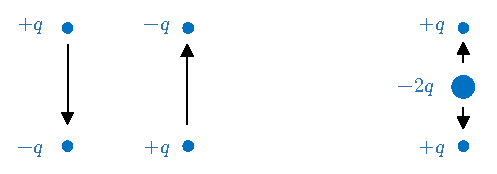
\includegraphics{elemental_quadrupoles.pdf}
			\caption{}
			\label{fig:elemental_quadrupoles}
		\end{figure}

		Es gibt zwei elementare Quadrupole (mit $\vec {p}=0$)

		Wird der Bezugspunkt/Aufpunkt verschoben, so ändern sich im Allgemeinen die Multipolmomente, aber das erste Moment, das bei der Multipolentwicklung einer Ladungsverteilung ungleich $0$ ist, bleibt unverändert.


		\begin{quote}
			Das niedrigste, nicht-verschwindende Multipolmoment in der Entwicklung ist unabhängig vom Bezugspunkt.
		\end{quote}
		Man kann natürlich auch sphärische Multipolmomente mithilfe von Kugelflächenfunktionen ausdrücken.

\end{enumerate}
\subsection{Energie von Multipolen im äußeren Feld\label{ref-034}}

Die Energie von Multipolen in einem externen Potential $\phi _{e}\left(\vec {r}\right)$ kann bereits bekannten Formel für die Energie einer beliebigen Ladungsverteilung $\rho \left(\vec {r}\right)$ abgeleitet werden:
\begin{equation*}
	U=\int _{V}\diff ^{3}\vec {r}\rho \left(\vec {r}\right)\phi _{e}\left(\vec {r}\right)
\end{equation*}
Wir nehmen an, dass die Änderung von $\phi _{e}$ in $V$ nur klein ist und erhalten durch eine Taylor-Entwicklung
\begin{equation*}
	U=\int \diff ^{3}\vec {r}\rho \left(\vec {r}\right)\left[\phi _{e}\left(0\right)+\vec {r}\nabla \phi _{e}\left(0\right)+\frac{1}{2}x_{i}x_{j}\nabla _{i}\nabla _{j}\phi _{e}\left(0\right)+\ldots \right]=q\phi \left(0\right)-\vec {p}\cdot E_{e}\left(0\right)-\frac{1}{6}Q_{ij}\nabla _{j}E_{e}^{\left(i\right)}\left(0\right)+\ldots
\end{equation*}
Die Energie der Multipole ist also durch die $n$-fache Ableitung des Potentials, $\nabla ^{n}\phi $ bestimmt. Diese Rechnung erlaubt wegen der Taylor-Entwicklung eine beliebige Wahl des Bezugspunkts.



\begin{figure}[htb]
	\centering
	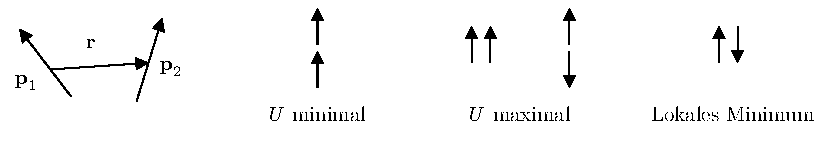
\includegraphics{dipoles.pdf}
	\caption{}
	\label{fig:dipoles}
\end{figure}

Als klassisches Beispiel soll die Wechselwirkung zweier Dipole betrachtet werden. Die potentielle Energie kann berechnet werden, indem der Dipol $\vec {p}_{2}$ wie oben beschrieben in das Feld des Dipols $\vec {p}_{1}$ gesetzt wird (oder umgekehrt):
\begin{equation*}
	U_{\mathrm{DD}}=-\vec {p}_{2}\cdot \vec {E}_{1}\left(\vec {r}\right)=-\frac{1}{4\pi \varepsilon _{0}}\frac{1}{r^{3}}\left(\frac{3\left(\vec {r}\cdot \vec {p}_{1}\right)\left(\vec {r}\cdot \vec {p}_{2}\right)}{r^{2}}-\vec {p}_{1}\cdot \vec {p}_{2}\right)
\end{equation*}
Diese wird minimale für $\vec {p}_{1}\parallel \vec {p}_{2}\parallel \vec {r}$ und maximal für $\vec {p}_{1}\parallel \vec {p}_{2}\bot \vec {r}$. Für antiparallele $\vec {p}_{1}$ und $\vec {p}_{2}$ und $\vec {p}_{1},\vec {p}_{2}\bot \vec {r}$ wird außerdem ein lokales Minimum erreicht. Aus diesem Grund bilden Dipolmoleküle auch häufig Molekülketten.

Zuletzt sollen noch Drehmomente auf Multipole diskutiert werden.
\begin{equation*}
	\begin{array}{ll}
		\vec {M}          & =\int \diff ^{3}\vec {r}\vec {r}\times \underset{\text{Kraftdichte}}{\underbrace{\rho \left(\vec {r}\right)\vec {E}_{e}\left(\vec {r}\right)}}\Rightarrow M_{i}=\int \diff ^{3}\vec {r}\varepsilon _{ijk}x_{j}\rho \left(\vec {r}\right)\underset{\approx E_{e}^{\left(k\right)}\left(0\right)+x_{l}\nabla _{l}E_{e}^{\left(k\right)}\left(0\right)}{\underbrace{E_{e}^{\left(k\right)}\left(\vec {r}\right)}} \\
		\Rightarrow M_{i} & =\left(\vec {p}\times \vec {E}_{e}\right)_{i}+\frac{1}{3}\varepsilon _{ijk}Q_{jl}\nabla _{l}E_{e}^{\left(k\right)}
	\end{array}
\end{equation*}
Insbesondere dreht das Drehmoment $\vec {M}$ einen Dipol parallel zu $\vec {E}$, da $\vec {M}=0$ für $\vec {p}\parallel \vec {E}_{e}$ und
\begin{equation*}
	U=-\vec {p}\cdot \vec {E}_{e}=-pE_{e}\cos \vartheta \Rightarrow M=-\frac{\partial U}{\partial \vartheta }=-pE_{e}\sin \vartheta =-\left| \vec {p}\times \vec {E}_{e}\right| .
\end{equation*}
\chapter{Elektrische Felder in Materie\label{ref-035}}

In diesem Kapitel werden makroskopischen Gleichungen der Elektrostatik in Materie beschrieben und erläutert.

\section{Mikroskopische Gleichungen der Elektrostatik und Mittelung\label{ref-036}}

Bis jetzt haben wir nur freie Ladungen betrachtet. Die Ladungsdichte $\rho \left(\vec {r}\right)$ erzeugt ein elektrisches Feld $\vec {E}$. In Materie sind zusätzliche auch gebundene Ladungen vorhanden, die mit dem Feld wechselwirken. Das können (nach außen hin elektrisch neutrale) Atome, geladenen Ionen, permanente Dipole (oder Multipole) sein (z.B. $\mathrm{H}_{2}\mathrm{O}$) sowie Dipole, die durch ein äußeres elektrisches Feld induziert werden.

Um diese Wechselwirkung zu beschrieben, wird eine Mittelung der mikroskopischen Gleichungen
\begin{equation*}
	\divg \vec {e}=\frac{1}{\varepsilon _{0}}\rho \left(\vec {r}\right),\quad \rot \vec {e}=0
\end{equation*}
durchgeführt. Wir haben bisher einzelne Ladungen durch $\delta $-Funktionen in der Ladungsdichte beschrieben. Dadurch kommt es zu starken räumlichen Ladungsschwankungen. Für eine makroskopische Betrachtung in Größenordnungen von Nanometern wenden wir eine räumliche Mittelung bzw. Glättungsfunktion auf die Ladungsdichteverteilung an.

\subsection{Glättungsfunktion\label{ref-037}}

Um eine stark variierende Funktion $F\left(\vec {r},t\right)$ zu mitteln, wird sie mit einer sogenannten Glättungsfunktion $f$ gefaltet. Dabei kann es sich z.B. um eine Gauß-Funktion handeln:
\begin{equation*}
	F\left(\vec {r},t\right) \overset{\text{Mittelung}}{\rightarrow } \left\langle F\left(\vec {r},t\right)\right\rangle =\int f\left(\left| \vec {r}-\vec {r}'\right| \right)F\left(\vec {r}',t\right)\diff ^{3}\vec {r}'
\end{equation*}
Betrachte als Beispiel eine Punktladung $F\left(\vec {r}\right)=F_{0}\delta \left(\vec {r}-\vec {r}_{0}\right)\rightarrow \left\langle F\right\rangle =F_{0}f\left(\vec {r}-\vec {r}_{0}\right)$.

Es gelten außerdem die folgenden Eigenschaften:\begin{enumerate}[1)]


	\item[1)] Die Mittelung der konstanten Funktion $F=1$ ist genau dann konstant $1$, wenn die Glättungsfunktion über den gesamten Raum auf $1$ normiert ist,
		\begin{equation*}
			\left\langle 1\right\rangle =1\Leftrightarrow \int \diff ^{3}\vec {r}f=1.
		\end{equation*}
	\item[2)] $\partial _{i}\left\langle F\right\rangle =\left\langle \partial _{i}F\right\rangle $.

\end{enumerate}
\section{Makroskopische Gleichungen der Elektrostatik\label{ref-038}}

Mithilfe der Glättung kann man das makroskopische $\vec {E}$-Feld als
\begin{equation*}
	\vec {E}\left(\vec {r},t\right)=\left\langle \vec {e}\left(\vec {r},t\right)\right\rangle
\end{equation*}
schreiben. Für die Ladungsdichte erhält man
\begin{equation*}
	\left\langle \rho \left(\vec {r}\right)\right\rangle =\left\langle \rho _{f}\left(\vec {r}\right)+\rho _{b}\left(\vec {r}\right)\right\rangle =\left\langle \rho _{f}\left(\vec {r}\right)\right\rangle +\left\langle \rho _{b}\left(\vec {r}\right)\right\rangle \equiv \rho _{F}+\rho _{B}.
\end{equation*}
Die gebundenen Ladungen werden als Summe der Ladungsdichten einzelner Moleküle geschrieben:
\begin{equation*}
	\rho _{b}\left(\vec {r}\right)=\sum _{n}\rho _{n}\left(\vec {r}\right), \rho _{n}\left(\vec {r}\right)=\sum _{i}q_{i}\delta \left(\vec {r}-\vec {r}_{i}\right)=\sum _{i}q_{i}\delta \left(\vec {r}-\left(\vec {r}_{n}+\vec {r}_{ni}\right)\right)
\end{equation*}
mit neuen Bezugspunkten $\vec {r}_{n}$ für die einzelnen Moleküle. Für die Mittelung wird dann eine Taylor-Entwicklung um diese neuen Bezugspunkte $\vec {r}_{n}$ verwendet:
\begin{align*}
	\left\langle \rho _{n}\left(\vec {r}\right)\right\rangle &=\sum _{i}q_{i}f\left(\vec {r}-\left(\vec {r}_{n}+\vec {r}_{ni}\right)\right)\\&=\sum _{i}q_{i}\left[f\left(\vec {r}-\vec {r}_{n}\right)-\vec {r}_{ni}\cdot \nabla f\left(\vec {r}-\vec {r}_{n}\right)+\frac{1}{2}\left(\vec {r}_{ni}\right)_{k}\left(\vec {r}_{ni}\right)_{l}\nabla _{k}\nabla _{l}f\left(\vec {r}-\vec {r}_{n}\right)+\ldots \right]
\end{align*}
Daraus können die molekularen Dipolmomente bestimmt werden:
\begin{align*}
		q_{n}                            & =\sum _{i}q_{i} \left(\text{Molekulare Ladung}\right)                                                                        \\
		\vec {p}_{n}                     & =\sum _{i}q_{i}\vec {r}_{ni} \left(\text{Molekulares Dipolmoment}\right)                                                     \\
		\left(\mathrm{Q}_{n}\right)_{kl} & =3\sum _{i}q_{i}\left(\vec {r}_{ni}\right)_{k}\left(\vec {r}_{ni}\right)_{l} \left(\text{Molekulares Quadrupolmoment}\right)
\end{align*}
(vgl. Multipolmomente einer kontinuierlichen Ladungsverteilung, aber hier diskret). Insgesamt ergibt sich eine Verschmierung punktförmiger molekularer Multipole:
\begin{align*}
	\left\langle \rho _{n}\left(\vec {r}\right)\right\rangle &=q_{n}f\left(\vec {r}-\vec {r}_{n}\right)-\vec {p}_{n}\cdot \nabla f\left(\vec {r}-\vec {r}_{n}\right)+\frac{1}{6}\left(\mathrm{Q}_{n}\right)_{kl}\nabla _{k}\nabla _{l}f\left(\vec {r}-\vec {r}_{n}\right) \\&=\left\langle q_{n}\delta \left(\vec {r}-\vec {r}_{n}\right)\right\rangle -\nabla \cdot \left\langle p_{n}\delta \left(\vec {r}-\vec {r}_{n}\right)\right\rangle +\frac{1}{6}\nabla _{k}\nabla _{l}\left\langle \left(\mathrm{Q}_{n}\right)_{kl}\delta \left(\vec {r}-\vec {r}_{n}\right)\right\rangle
\end{align*}
und für die gemittelte gebundene Ladungsdichte:
\begin{equation*}
	\left\langle \rho _{b}\left(\vec {r}\right)\right\rangle =\rho _{\mathrm{m}}\left(\vec {r}\right)-\nabla \cdot \vec {P}\left(\vec {r}\right)+\nabla _{k}\nabla _{l}\mathrm{Q}_{\mathrm{kl}}+\ldots
\end{equation*}
mit der makroskopischen Ladungsdichte (Monopoldichte)
\begin{equation*}
	\rho _{\mathrm{m}}\left(\vec {r}\right)=\left\langle \sum _{n}q_{n}\delta \left(\vec {r}-\vec {r}_{n}\right)\right\rangle ,
\end{equation*}
der Polarisation (Dipolmomentdichte)
\begin{equation*}
	\vec {P}\left(\vec {r}\right)=\left\langle \sum _{n}\vec {p}_{n}\delta \left(\vec {r}-\vec {r}_{n}\right)\right\rangle
\end{equation*}
und so weiter.

